\documentclass{article}

\usepackage{graphicx}
\usepackage{geometry}
 \geometry{
 a4paper,
 total={170mm,257mm},
 left=20mm,
 top=20mm,
 }

\begin{document}

\centering

\section{Optimized Parameters}

\begin{figure}[h!]
\centering
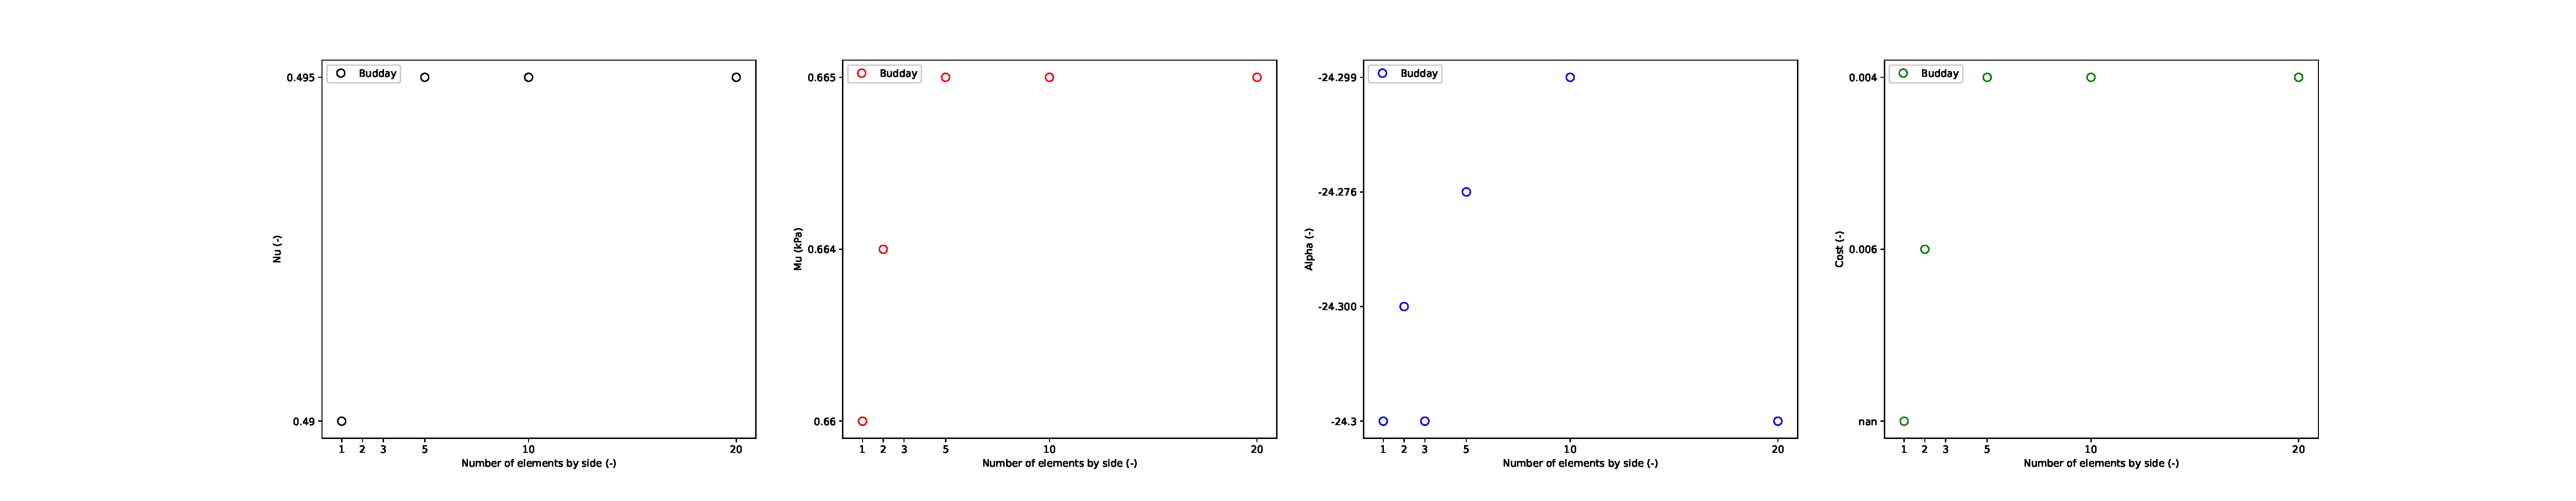
\includegraphics[width=1\linewidth, trim= 250 0 250 0]{OptimizedParametersFixedNeo-Hookean}
\caption{Fixed boundary conditions, Neo-Hookean Model}
\end{figure}

\begin{figure}[h!]
\centering
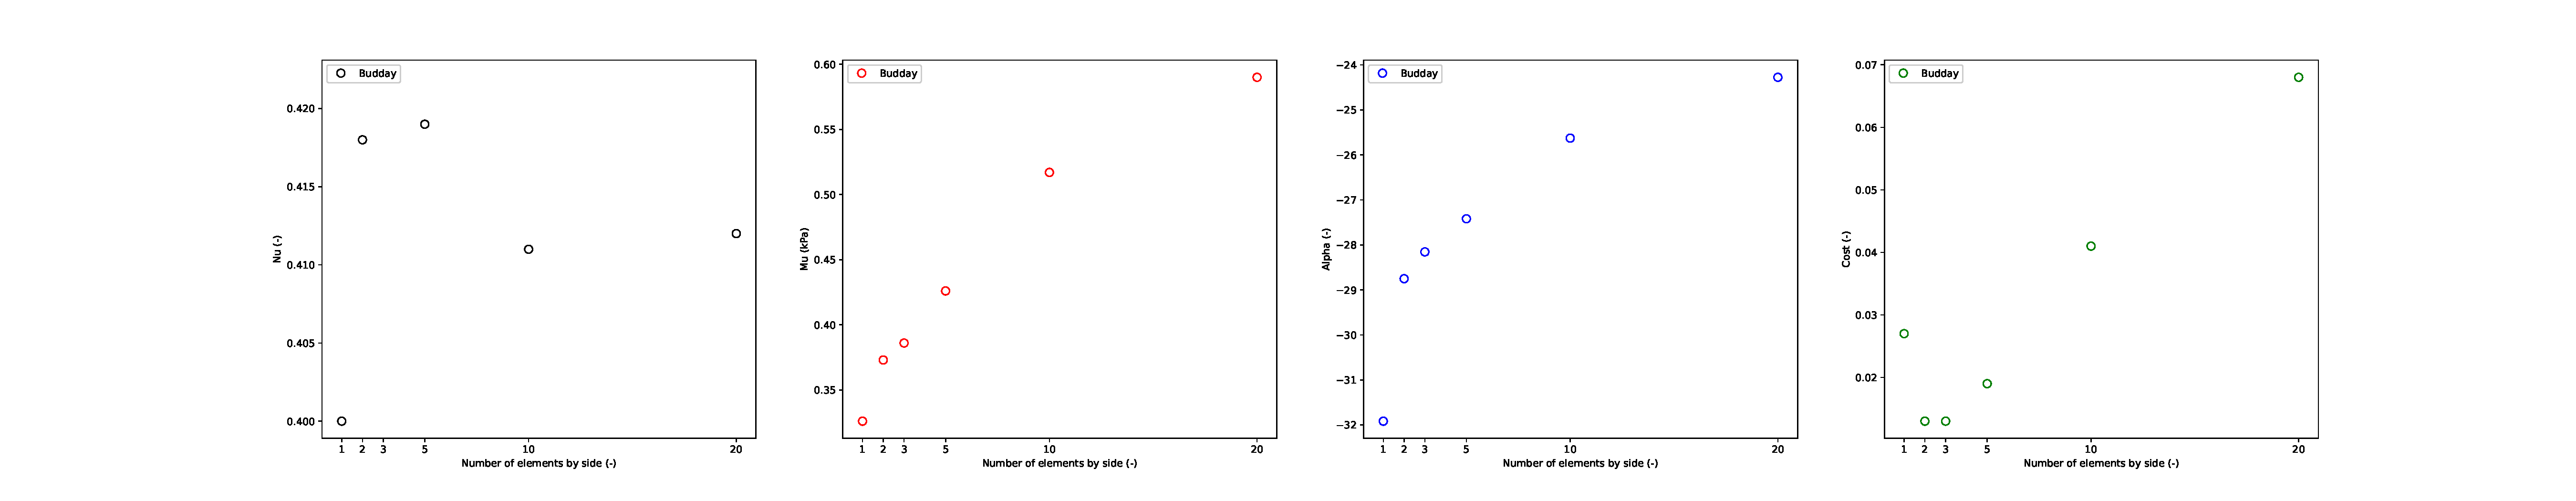
\includegraphics[width=\linewidth, trim= 250 0 250 0]{OptimizedParametersFixedOgden}
\caption{Fixed boundary conditions, Ogden Model}
\end{figure}

\begin{figure}[h!]
\centering
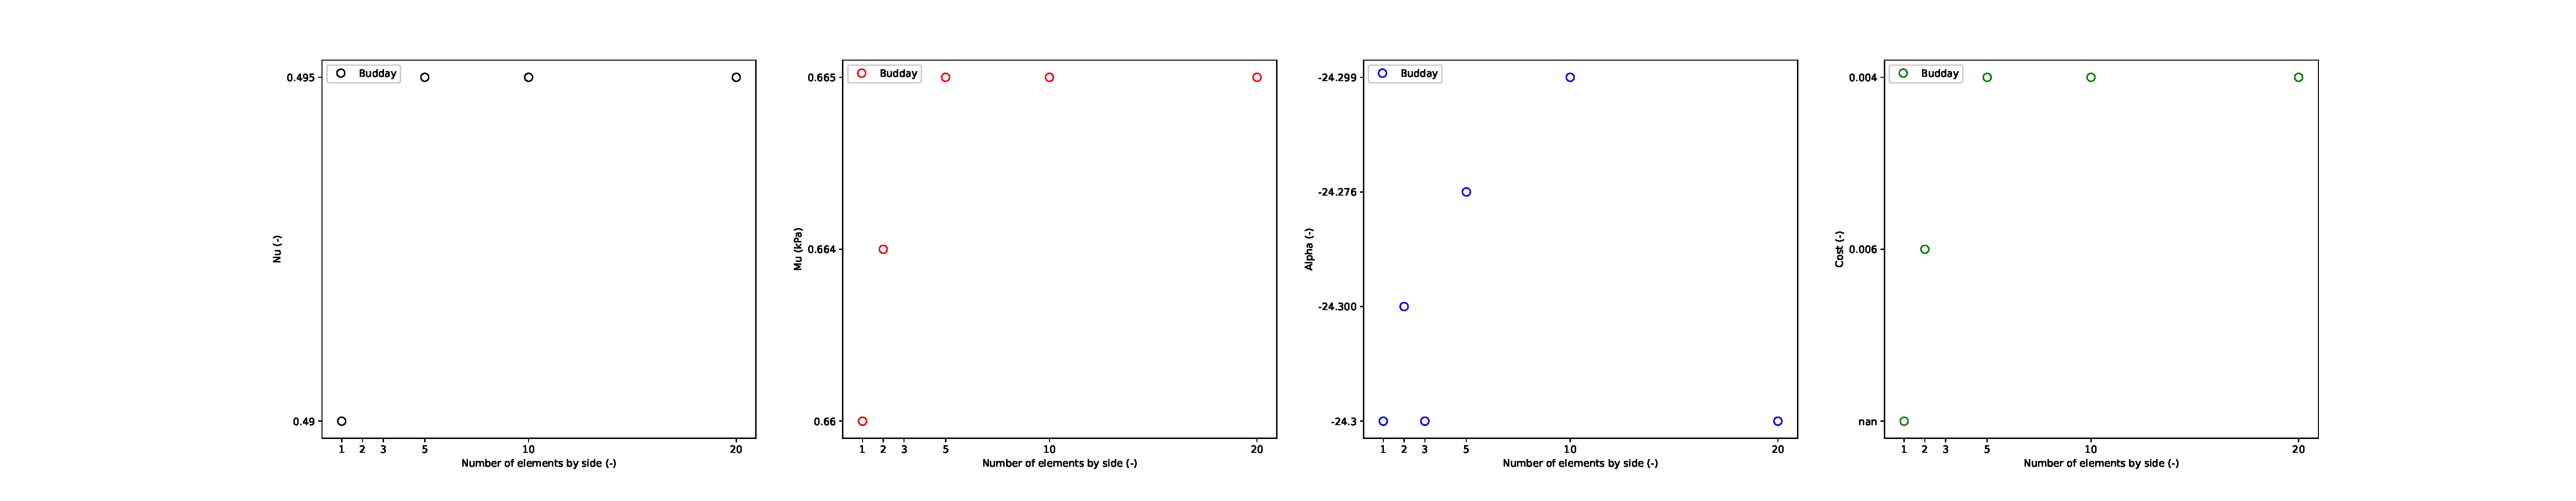
\includegraphics[width=\linewidth, trim= 250 0 250 0]{OptimizedParametersIdealNeo-Hookean}
\caption{Ideal boundary conditions, Neo-Hookean Model}
\end{figure}

\begin{figure}[h!]
\centering
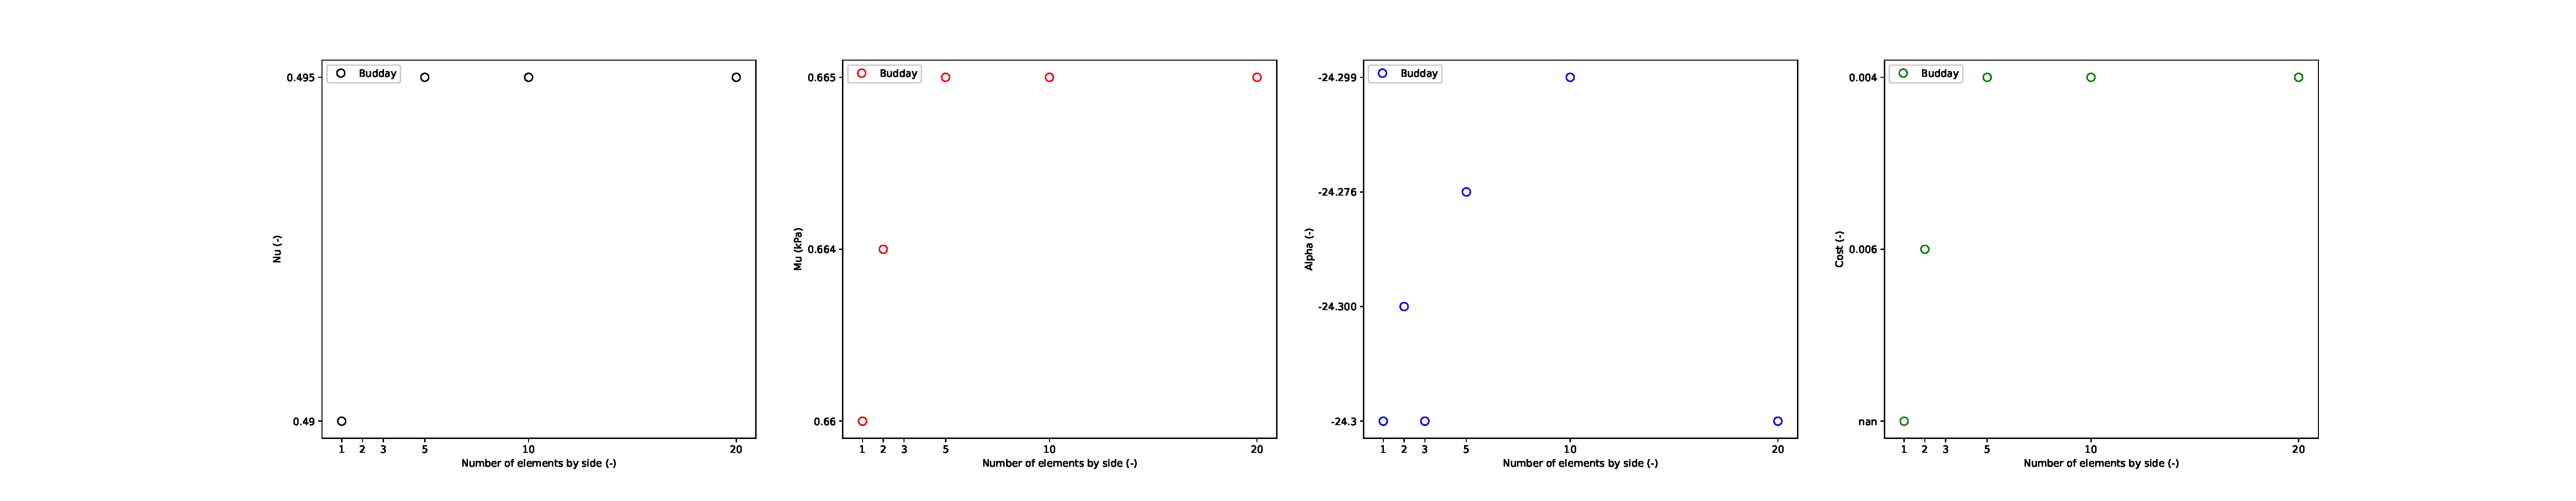
\includegraphics[width=\linewidth, trim= 250 0 250 0]{OptimizedParametersIdealOgden}
\caption{Ideal boundary conditions, Ogden Model}
\end{figure}

\newpage

\section{Parameters Evolution}

\centering
\begin{figure}[h!]
\centering
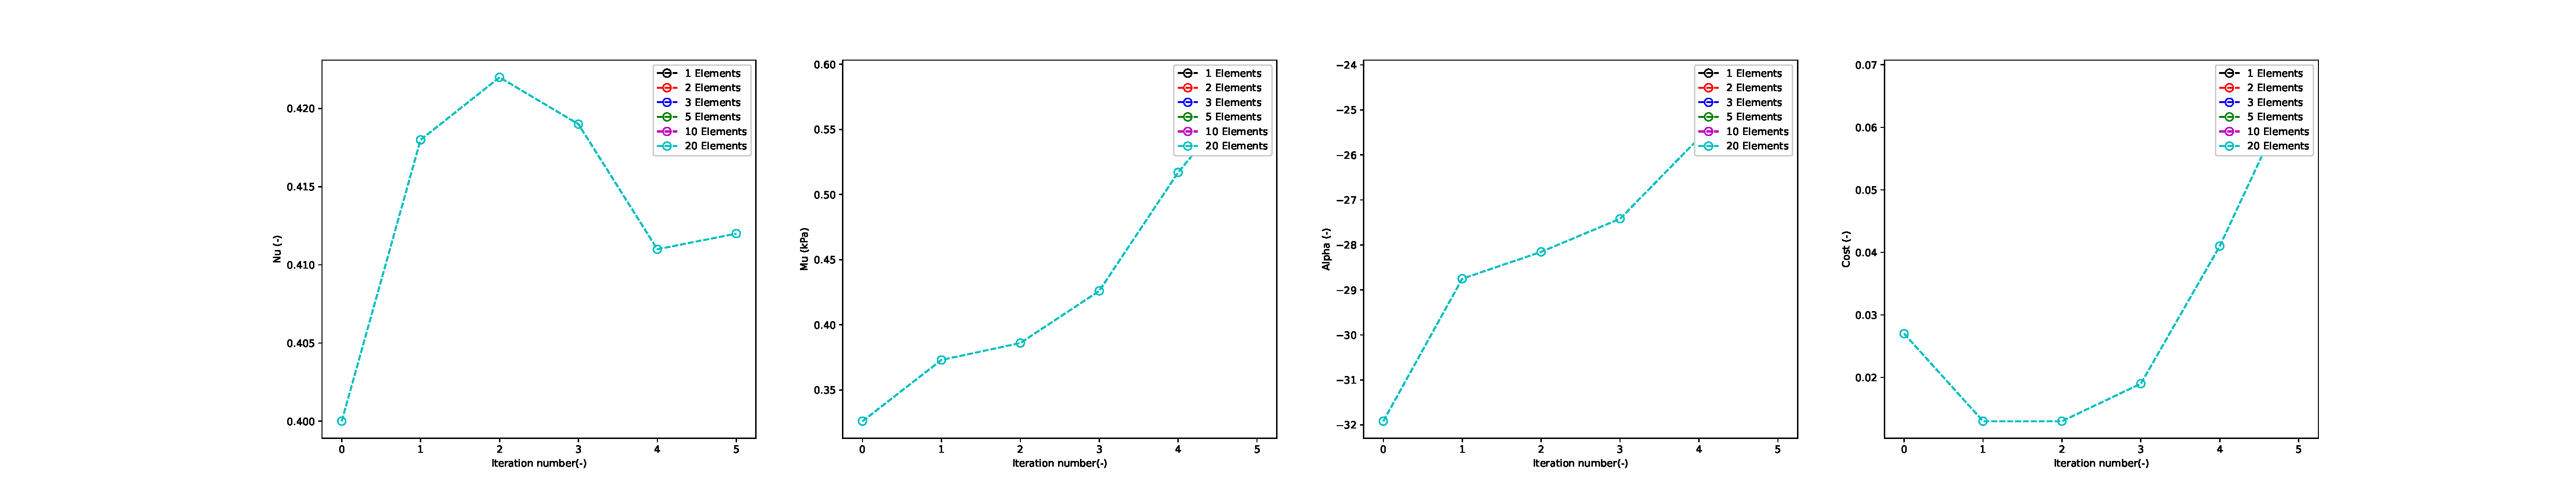
\includegraphics[width=1\linewidth, trim= 250 0 250 0]{ParametersEvolutionFixedNeo-Hookean}
\caption{Fixed boundary conditions, Neo-Hookean Model}
\end{figure}

\begin{figure}[h!]
\centering
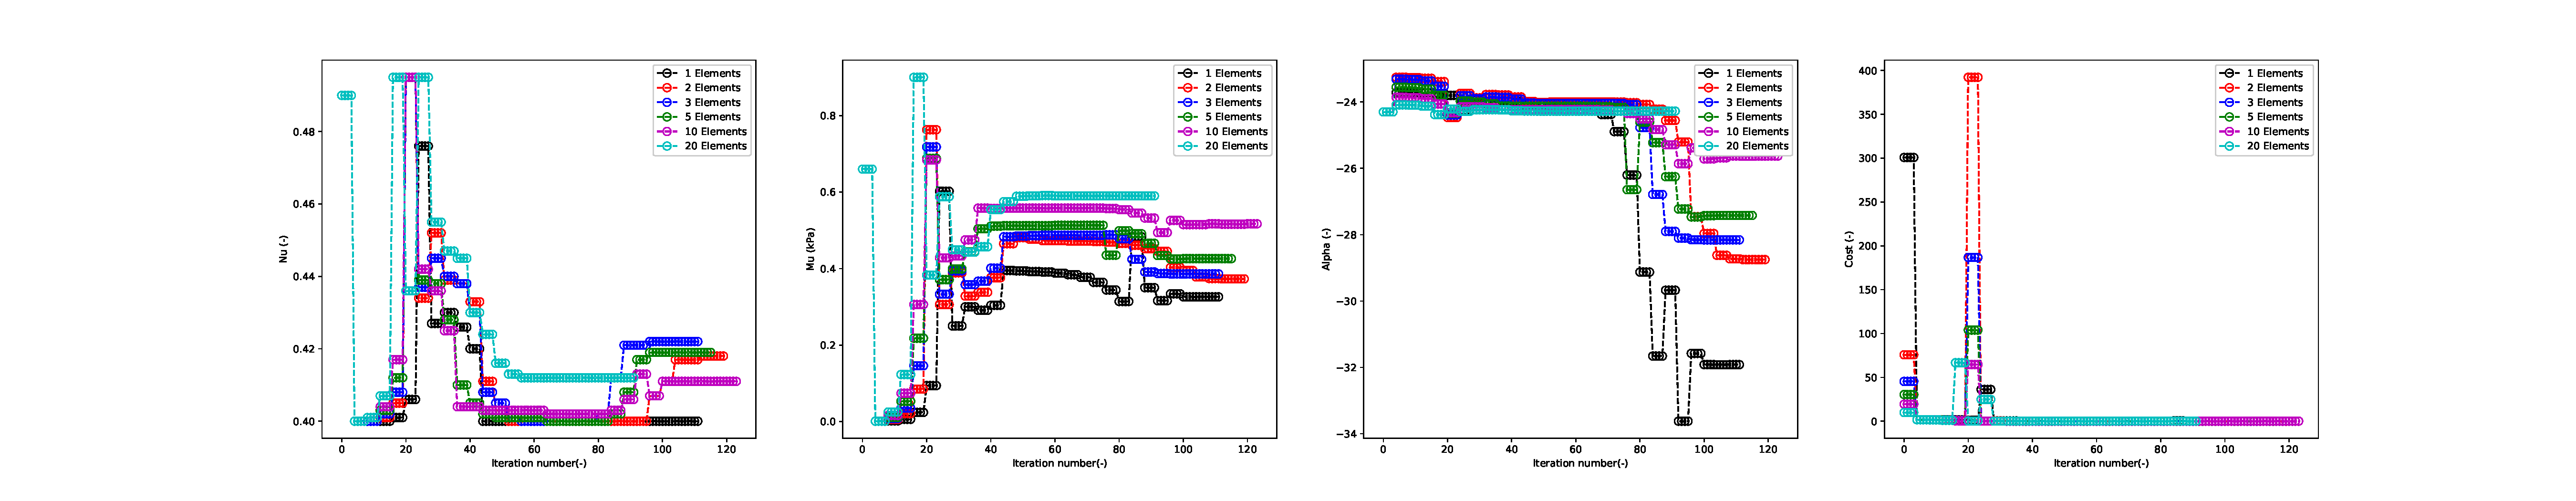
\includegraphics[width=\linewidth, trim= 250 0 250 0]{ParametersEvolutionFixedOgden}
\caption{Fixed boundary conditions, Ogden Model}
\end{figure}

\begin{figure}[h!]
\centering
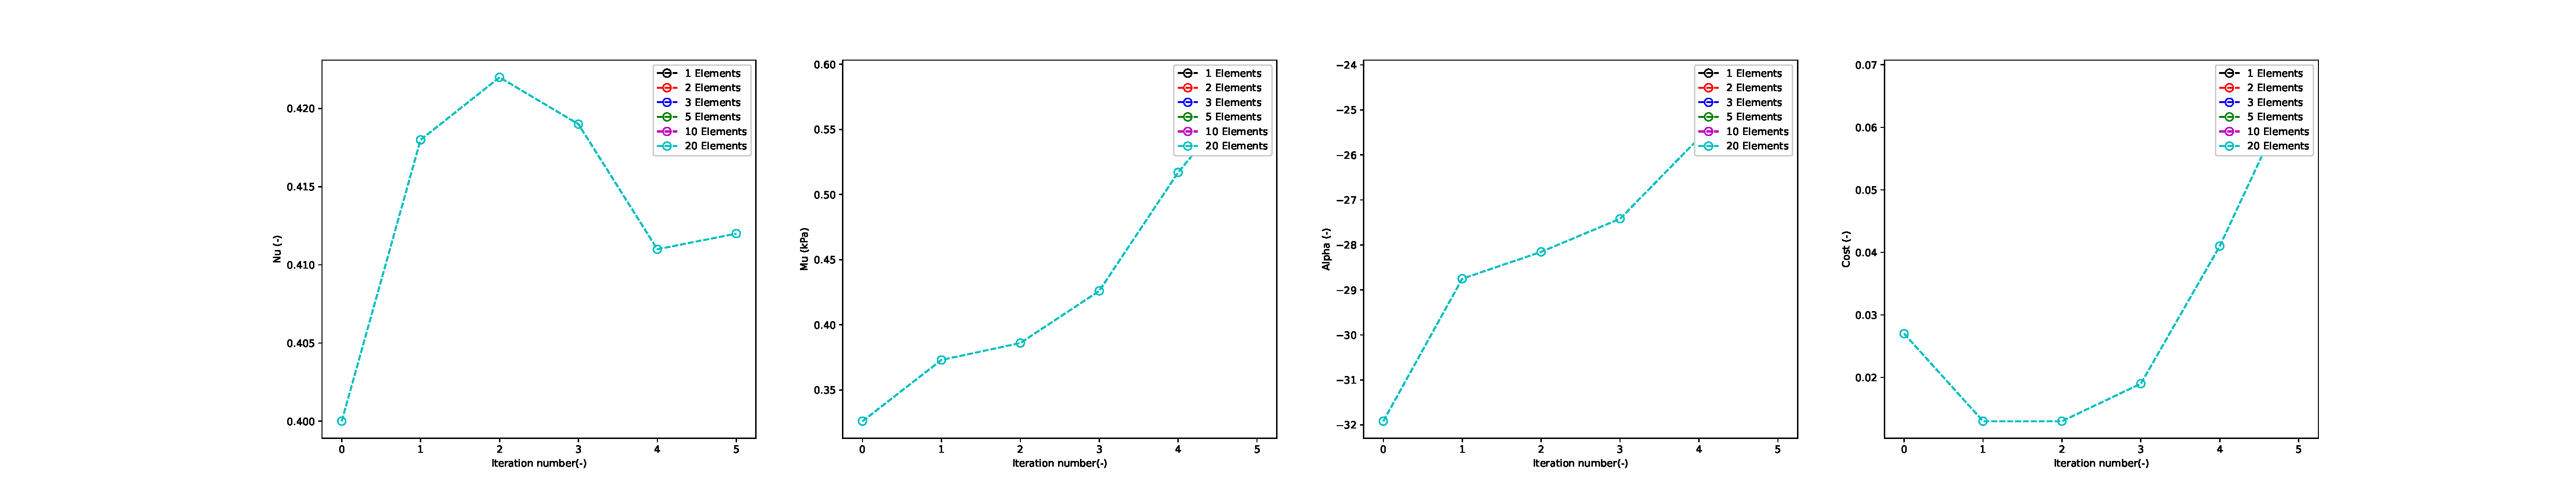
\includegraphics[width=\linewidth, trim= 250 0 250 0]{ParametersEvolutionIdealNeo-Hookean}
\caption{Ideal boundary conditions, Neo-Hookean Model}
\end{figure}

\begin{figure}[h!]
\centering
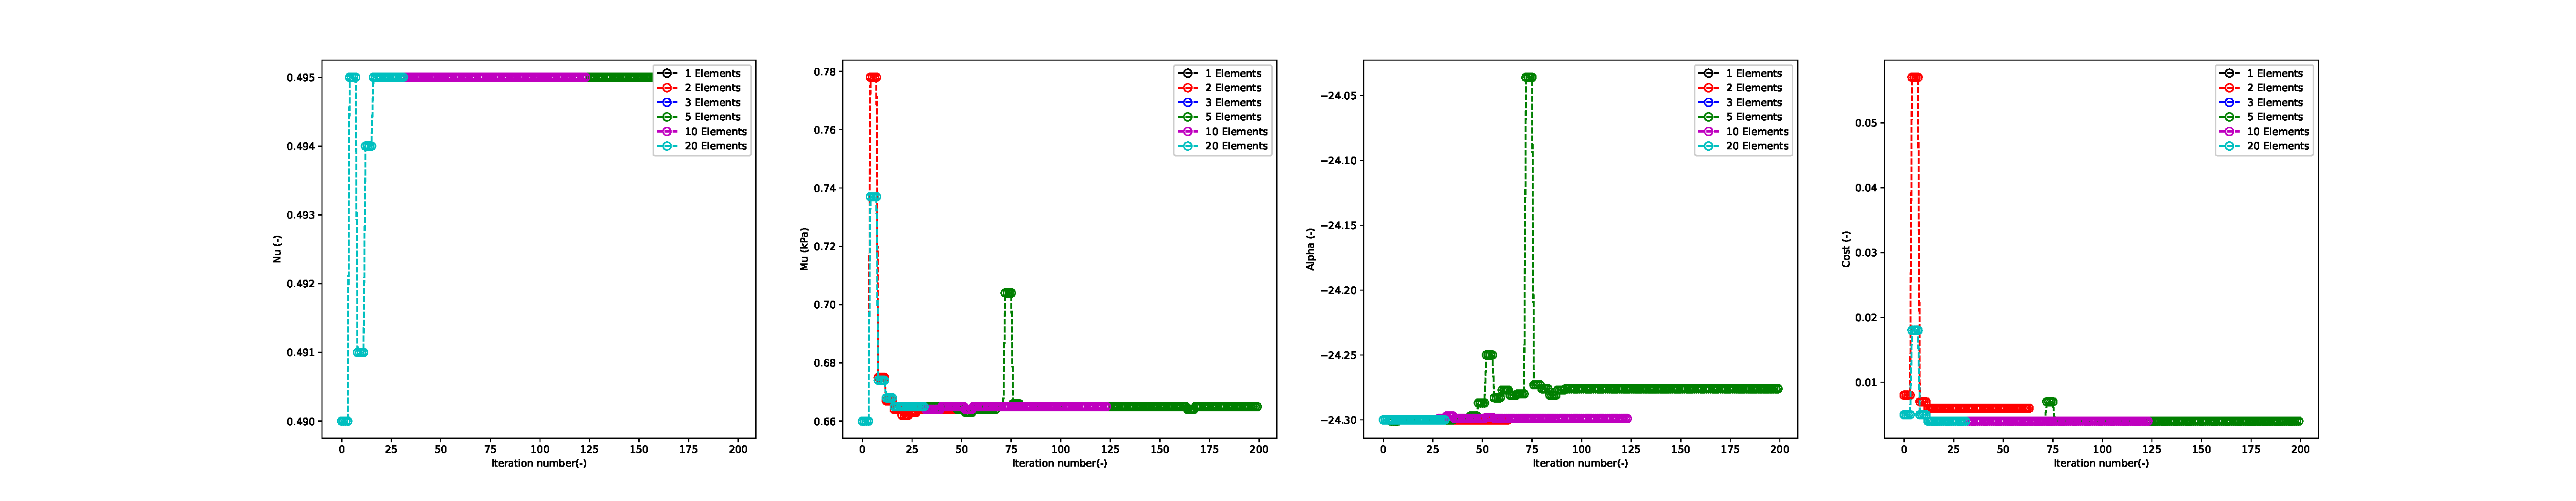
\includegraphics[width=\linewidth, trim= 250 0 250 0]{ParametersEvolutionIdealOgden}
\caption{Ideal boundary conditions, Ogden Model}
\end{figure}

\newpage

\section{Sensitivity}

\centering
\begin{figure}[h!]
\centering
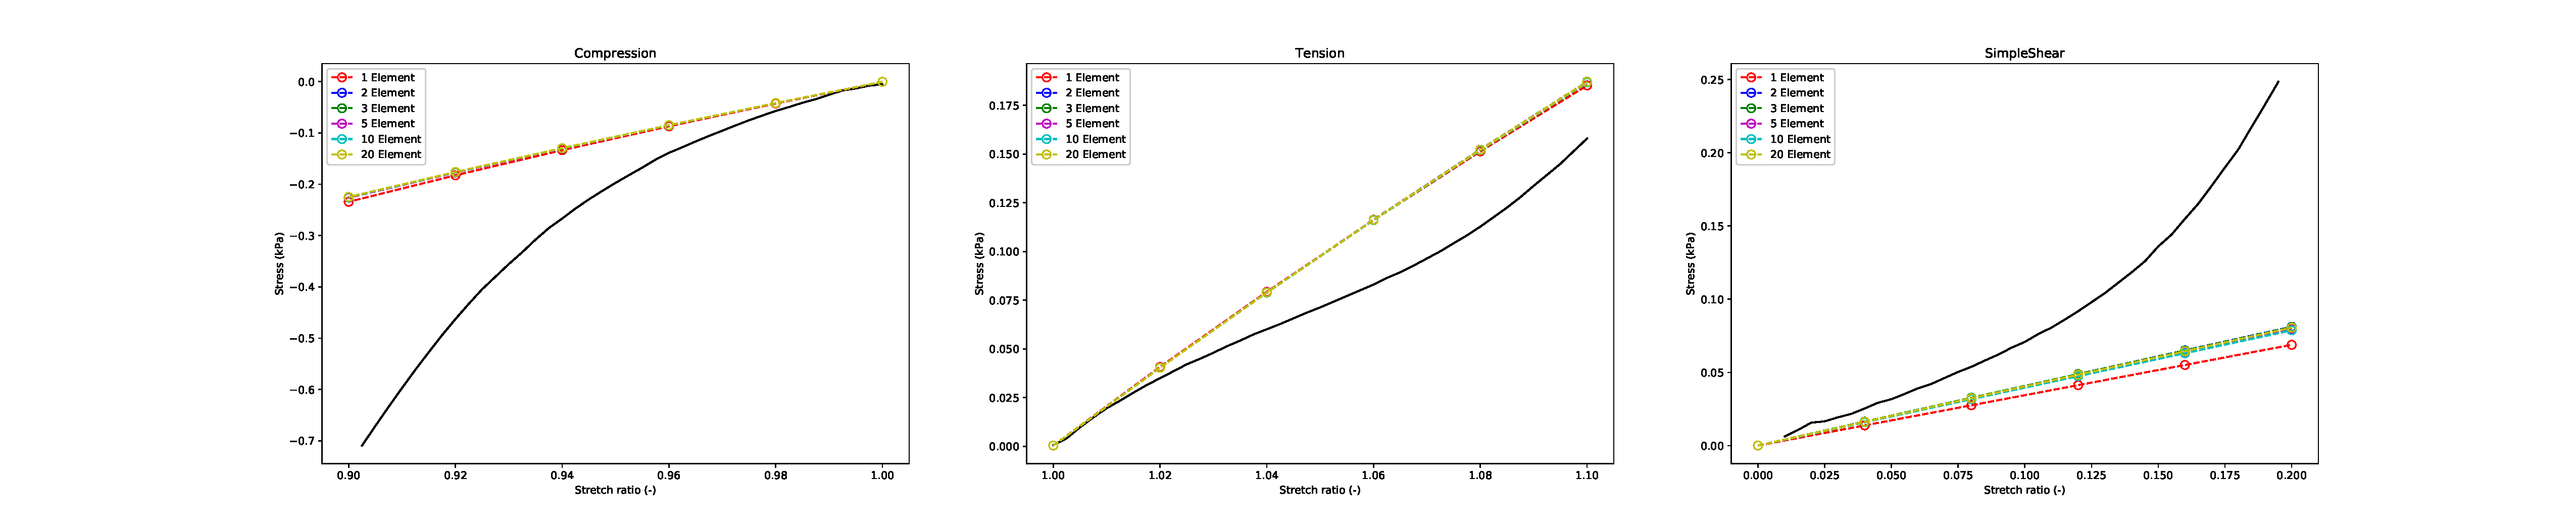
\includegraphics[width=1\linewidth, trim= 250 0 250 0]{SensitivityFixedNeo-Hookean}
\caption{Fixed boundary conditions, Neo-Hookean Model}
\end{figure}

\begin{figure}[h!]
\centering
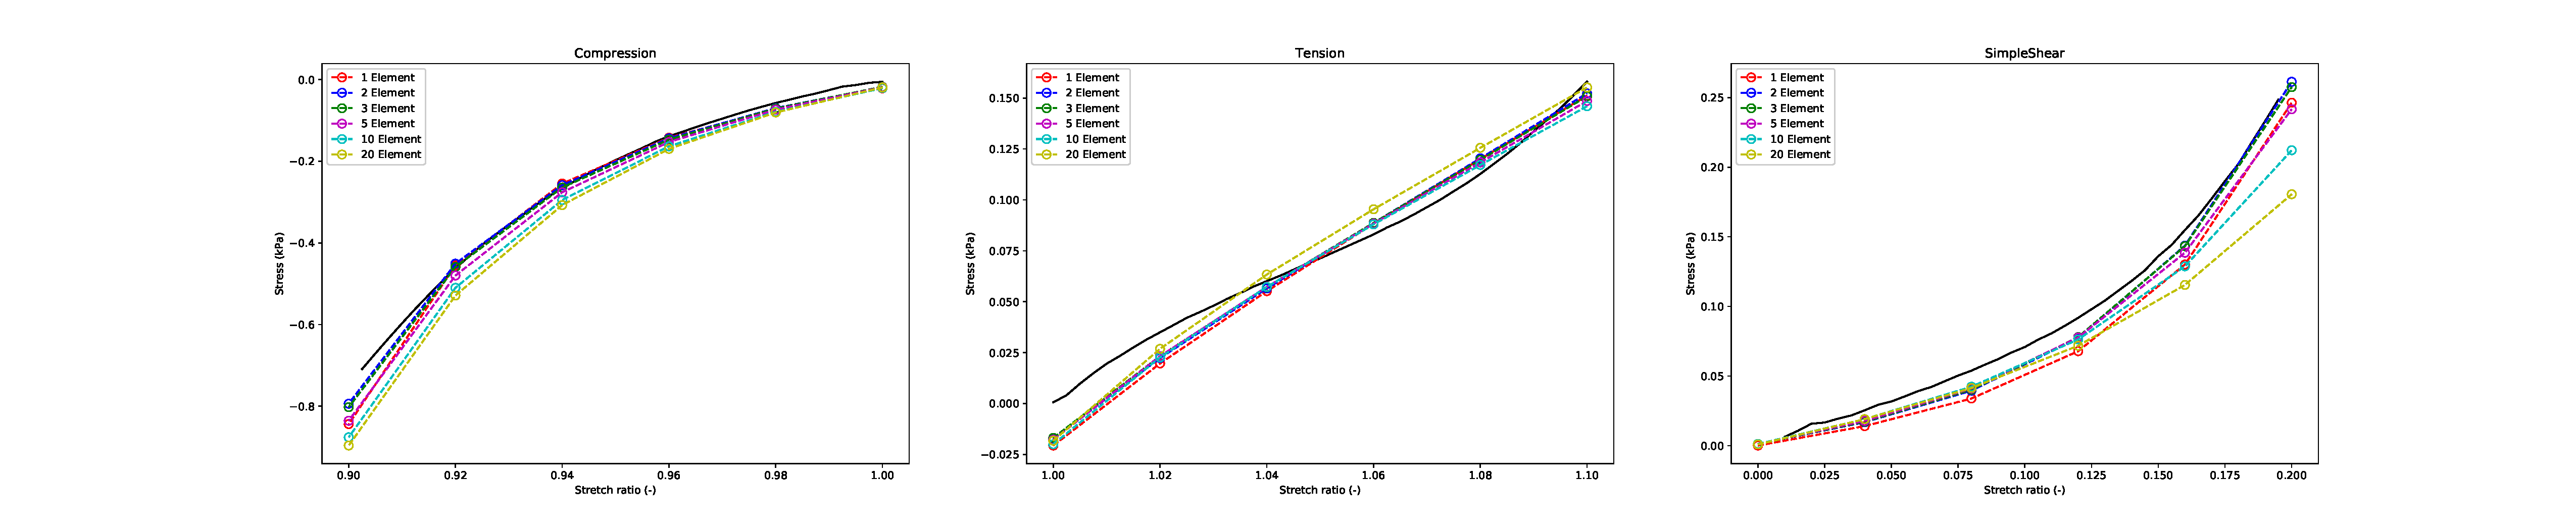
\includegraphics[width=\linewidth, trim= 250 0 250 0]{SensitivityFixedOgden}
\caption{Fixed boundary conditions, Ogden Model}
\end{figure}

\begin{figure}[h!]
\centering
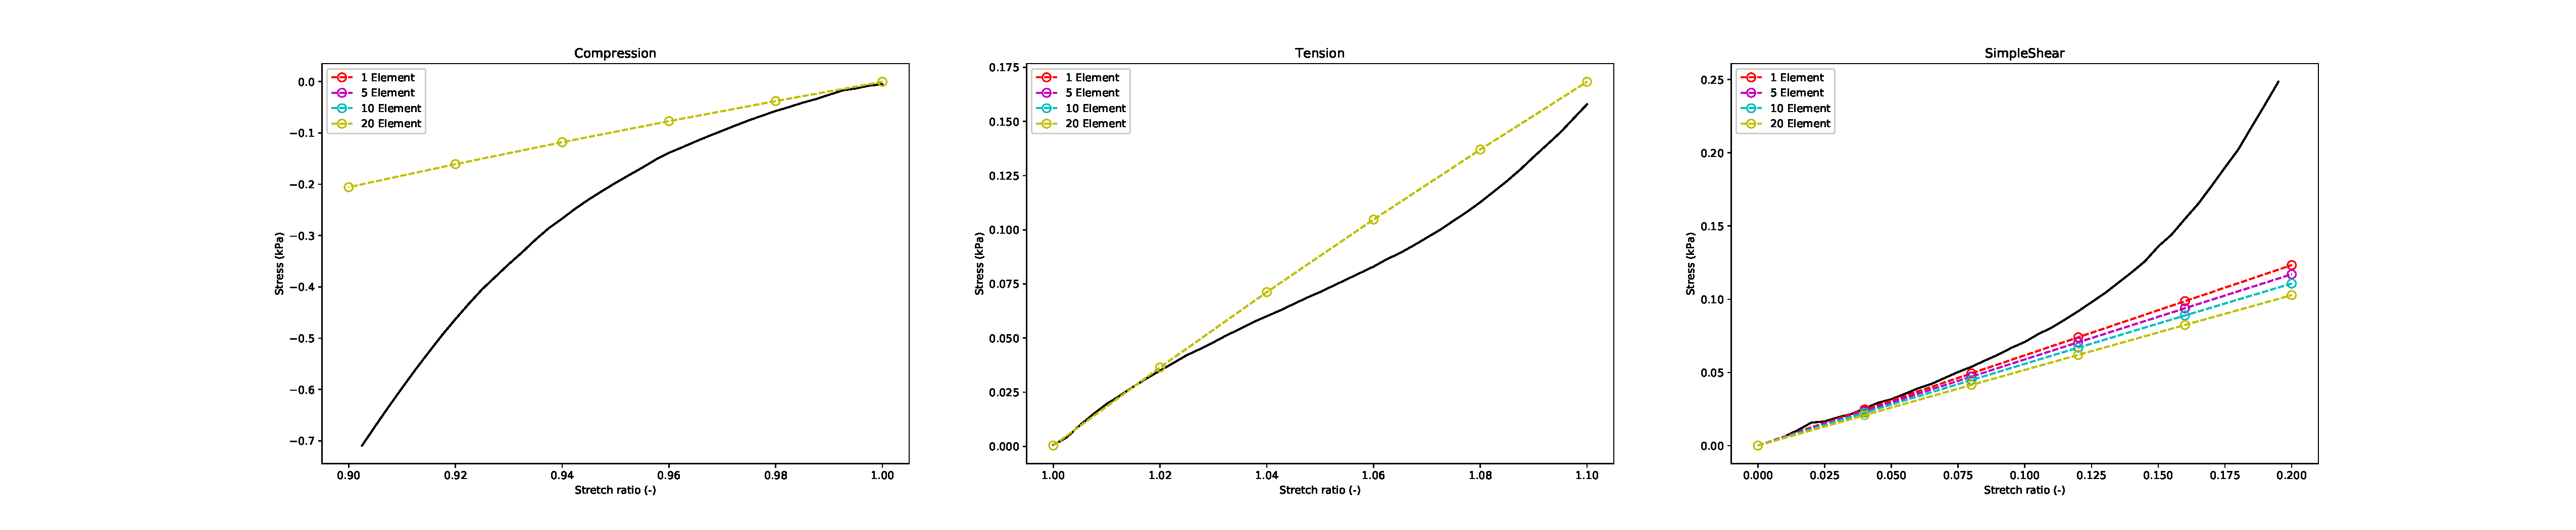
\includegraphics[width=\linewidth, trim= 250 0 250 0]{SensitivityIdealNeo-Hookean}
\caption{Ideal boundary conditions, Neo-Hookean Model}
\end{figure}

\begin{figure}[h!]
\centering
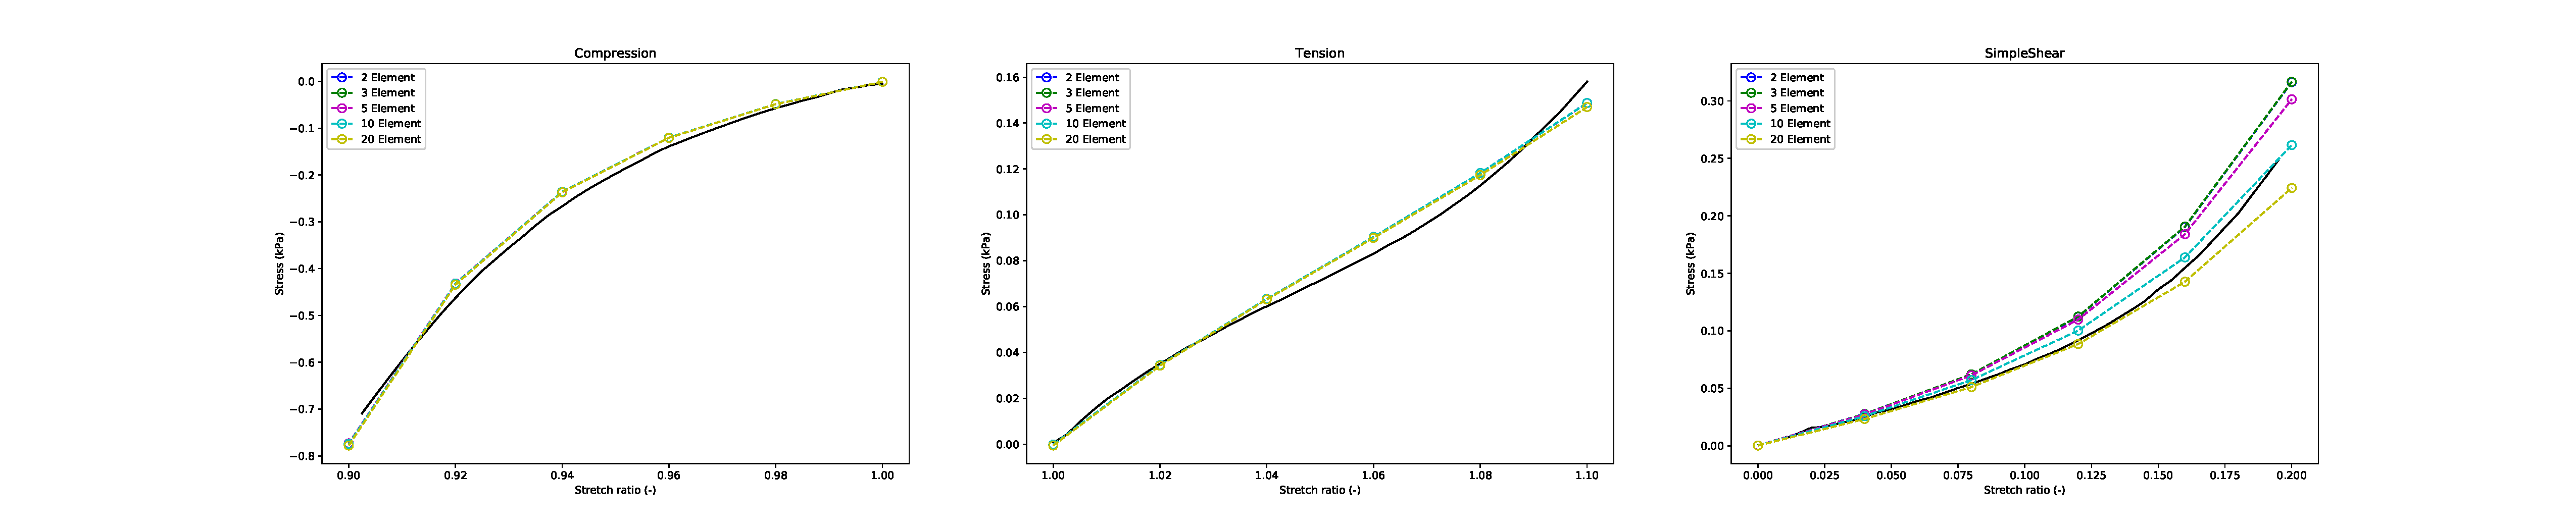
\includegraphics[width=\linewidth, trim= 250 0 250 0]{SensitivityIdealOgden}
\caption{Ideal boundary conditions, Ogden Model}
\end{figure}

\end{document}